\documentclass[a4paper,12pt]{article}
\usepackage[utf8]{inputenc}
\usepackage{graphicx}
\usepackage{fancyhdr}
\usepackage[left=2.5cm, right=2.5cm, top=3cm, bottom=3cm]{geometry}
\usepackage{adjustbox}
\usepackage{hyperref}
\graphicspath{{Imagenes/}}
\usepackage[backend=biber]{biblatex}
\bibliography{bibliografia}
% Aquí se asume que el archivo se llama "referencias.bib"

% Contenido del informe


% Encabezado y pie de página
\pagestyle{fancy}
\fancyhf{}
\setlength{\headheight}{30 pt}
\renewcommand{\headrulewidth}{0.2pt}
\fancyhead[L]{\begin{tabular}{@{}l@{}}
\includegraphics[scale=0.4]{escudo.PNG}\end{tabular}}
\fancyhead[R]{\begin{tabular}{@{}c@{}} \textbf{Programación Orientada a Objetos} \\ Parte A: Introducción a C++ \end{tabular}}



\fancyfoot[L]{\begin{tabular}{@{}l@{}}\includegraphics[scale=0.4]{año.PNG}\end{tabular}}
\fancyfoot[R]{\thepage}
\fancyfoot[C]{\begin{tabular}{@{}c@{}}\textbf{BORQUEZ PEREZ Juan Manuel}\\ \textbf{Legajo 13567}\end{tabular}}
\renewcommand{\footrulewidth}{0.2pt}

\begin{document}

\begin{titlepage}
    \centering
    \vspace*{5cm}
    {\Huge\bfseries Informe de Trabajo Práctico}\\
    \vspace{0.2cm}
    {\Large \textbf{N°1 - Parte A: Introducción a C++}}\\
    \vspace{0.5cm}
    {\Large Programación Orientada a Objetos}\\
    \vspace{0.2 cm}
    {\Large Ingeniería en Mecatrónica}\\
    \vspace{1.5cm}
    Alumno: Juan Manuel BORQUEZ PEREZ\\
    Legajo: 13567\\
    \vfill
    {\begin{tabular}{@{}c@{}}
\includegraphics[scale=0.4]{escudo.PNG}\end{tabular}}\hspace{10pt}
    {\begin{tabular}{@{}c@{}}\includegraphics[scale=0.6]{año.PNG}\end{tabular}}
    %Año 2023
\end{titlepage}
\section{Consignas}
\begin{itemize}
    \item[a)] Prepare un directorio denominado \texttt{apellido\_legajo\_A} (reemplace con sus datos) que contenga
    2 subdirectorios denominados \texttt{version\_anterior} y \texttt{version\_nueva}.
    
    \item[b)] Seleccione 1 ejercicio de los desarrollados en la asignatura Informática usando lenguaje C
    bajo paradigma estructurado y cópielo en el subdirectorio \texttt{version\_anterior}. El ejercicio elegido
    debe satisfacer el siguiente requerimiento:
    \begin{itemize}
        \item Presentar operaciones de entrada/salida por consola.
        \item Realizar al menos 2 tareas específicas.
        \item Tomar decisiones lógicas en base a expresiones y/o variables.
        \item Definir al menos 1 estructura de datos mediante \texttt{enum} o \texttt{struct}.
        \item Usar, al menos, una colección de datos (arreglo, lista, cola, árbol, etc.).
    \end{itemize}
    
    \item[c)] En el directorio \texttt{version\_nueva}, implemente la misma solución pero adaptando la
    implementación a las características generales propias de C++. Esta adaptación implica que:
    \begin{itemize}
        \item Cada tarea específica debe implementarse en una función que maneje argumentos adecuados.
        \item Las funciones que se definan deben ser consistentes en su diseño y reforzar la cohesión general.
        \item Se elimine toda macro y/o variable global (excepto las macros de guarda).
        \item Las variables usadas para almacenar datos lógicos deben declararse booleanas.
        \item Todos los datos numéricos que se visualicen en pantalla deben hacerlo usando 2 dígitos de precisión y, si corresponde, debidamente encolumnados (utilice como ayuda el código del programa \texttt{ajustar\_numeros.cpp}).
    \end{itemize}
    
    \item[d)] Verifique que, en las primeras líneas de cada archivo de la nueva versión (\texttt{.h}, \texttt{.hpp}, \texttt{.cpp}), se incorpore información similar a la siguiente:
    \begin{verbatim}
    /**
    * @package agregar_si_corresponde
    * Incluya aqui el objetivo del programa, por ejemplo:
    * Aplicacion y Host RPC para control de robots
    * del tipo brazo articulado con 3 grados de libertad.
    *
    * @version 1.0
    * @date 2023.08.11
    * @author Cesar Omar Aranda
    * @contact cesar.aranda@ingenieria.uncuyo.edu.ar
    * @see https://youtu.be/gu-gkutfFFo
    * @see https://youtu.be/qFtGcYrb1a4
    * @see https://youtu.be/qFtGcYrb1a4
    * @see https://www.thingiverse.com/thing:3674358
    * @see https://github.com/CesarAranda/HostCLI_RobotArm
    */
    \end{verbatim}

    \item[e)] Documente, brevemente cada función implementada. Suponiendo que la función sea:
    \begin{verbatim}
    double sumar(std::vector<double> & const valores) {
        ……
    }
    \end{verbatim}
    Agregue inmediatamente antes de la instrucción anterior, un texto similar a:
    \begin{verbatim}
    /**
    * Suma los números almacenados en un vector.
    *
    * @param valores Es el contenedor de los valores a ser sumados.
    * @returns la suma de los `valores`, o 0.0 si `valores` está vacío.
    */
    \end{verbatim}
    
    \item[f)] Elabore un informe que documente básicamente la implementación realizada. Salvo
    indicaciones adicionales que puedan darse en clase, el mismo debe contener2:
    \begin{itemize}
        \item Carátula: donde consten los datos de identificación personales y de contexto.
        \item Introducción/enunciado.
        \item Esquema general de la solución: representación gráfica con el diseño del modelo lógico.
        \item Interfaces de usuario: captura de pantallas de entrada/salida resultantes para una ejecución completa.
        \item Uso: descripción de las consideraciones a tener en cuenta por un usuario que desea hacer uso del aplicativo resultante y/o reutilizar su código.
        \item Conclusiones:
        \begin{itemize}
            \item Comentario sobre los cambios realizados, las dificultades encontradas, las particularidades de la implementación y/o conceptos que requieran atención especial.
            \item Comentario indicando de qué manera puede ser extendido cada uno de los temas del trabajo (si corresponde). \textbf{N/A}
            \item Resumen de observaciones/valoración personal a trabajo realizado. \textbf{N/A}
        \end{itemize}
        \item Referencias bibliográficas y URL (a sitios web, documentos, etc.) consultados.
        \item Anexos.
    \end{itemize}
    
    \item[g)] En la carpeta raíz (\texttt{apellido\_legajo\_A}) coloque el documento (en formato PDF preferentemente) con el informe asociado.
    
    \item[h)] Suba un archivo comprimido de la carpeta raíz creada (incluyendo todo su contenido) en la actividad denominada Entrega A, dentro del aula virtual.
\end{itemize}

\subsection{Consigna del ejercicio del Trabajo Práctico de Informática elegido}
Se escogió el ejercicio 5 de la Parte 1 - "Estructuras de Datos y Cadenas" del Trabajo Práctico N°3 de Informática, cuya consigna es la siguiente:

\begin{itemize}
    \item[5.]Modifique el ejercicio 12 del práctico anterior (el de las fechas) utilizando un \texttt{struct} que represente una fecha completa. Realice al menos una función que reciba por parámetro una fecha. Defina la estructura \texttt{fecha} como un tipo definido por el usuario (\texttt{typedef}).
\end{itemize}

El ejercicio al que se hace referencia en el enunciado es al ejercicio 12 de la Parte 3 - "Subrutinas" del Trabajo Práctico N°2 de Informática, cuya consigna es la siguiente:

\begin{itemize}
    \item[12.] Escribir un programa que le pida al usuario una fecha del estilo DD/MM/AAAA y determine:
\end{itemize}
\begin{enumerate}
    \item[a.] El día anterior y posterior.
    \item[b.] El último día del mes y cuántos días faltan para el mismo.
\end{enumerate}

\textbf{Considerar la existencia de los años bisiestos.}
\vspace{1cm}

\textbf{Los archivos con las consignas de los mencionados trabajos prácticos se encuentran cargados en el directorio "version\_anterior"}
\newpage
\section{Esquema General de la Solución}
\begin{figure}[!h]
    \centering
    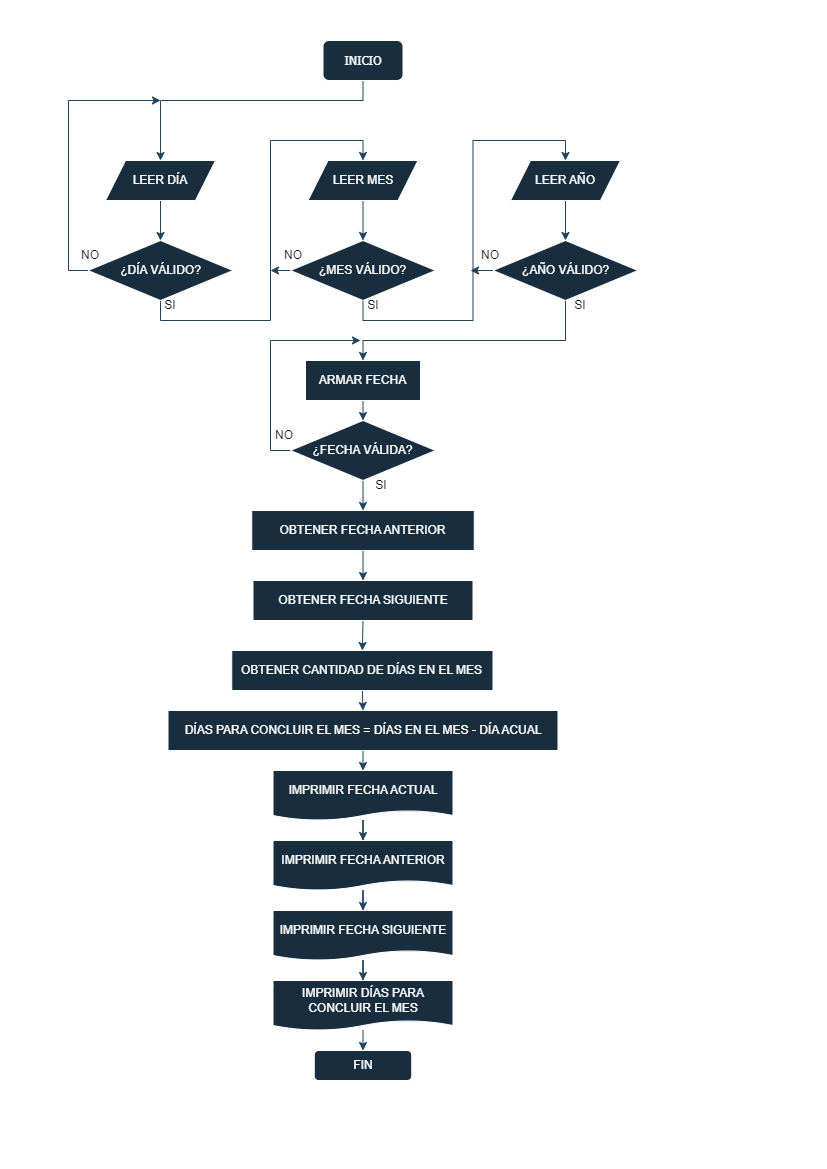
\includegraphics[width=\dimexpr\textwidth-4cm,height=\dimexpr\textheight-4cm]{Diagrama de Flujo del Programa.png}
\end{figure}
\newpage
\section{Interfaces de Usuario}
Secuencia de capturas para una ejecución completa
\begin{figure}[!ht]
    \centering
    \begin{adjustbox}{max width=\textwidth, center}
        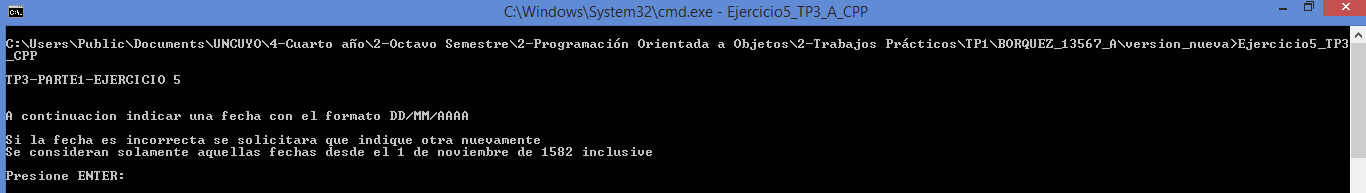
\includegraphics{Captura_UI_1.PNG}
    \end{adjustbox}
    \centering
    \begin{adjustbox}{max width=\textwidth, center}
        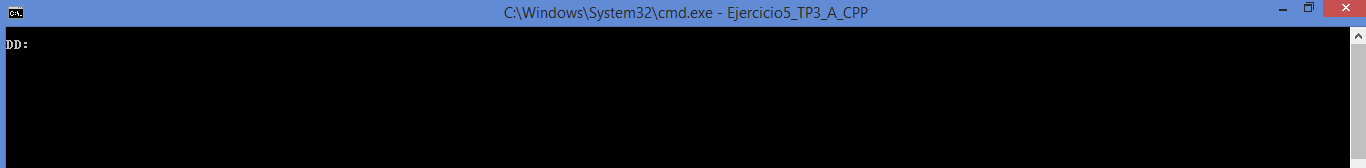
\includegraphics{Captura_UI_2.PNG}
    \end{adjustbox}
    \centering
    \begin{adjustbox}{max width=\textwidth, center}
        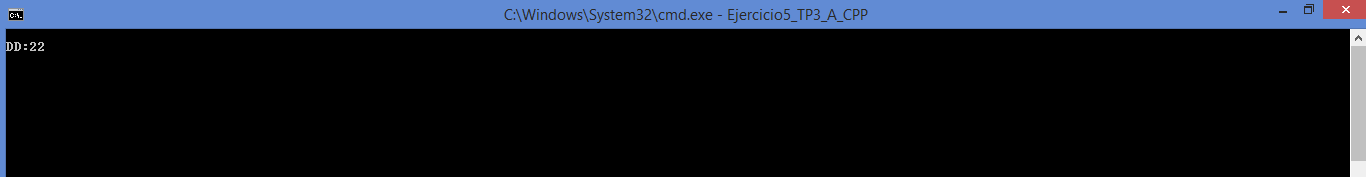
\includegraphics{Captura_UI_3.PNG}
    \end{adjustbox}
    \centering
    \begin{adjustbox}{max width=\textwidth, center}
        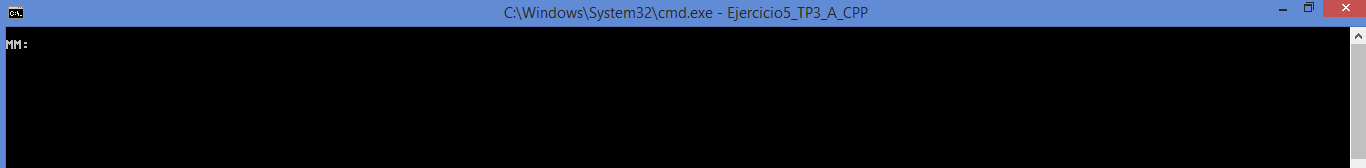
\includegraphics{Captura_UI_4.PNG}
    \end{adjustbox}
    \begin{adjustbox}{max width=\textwidth, center}
        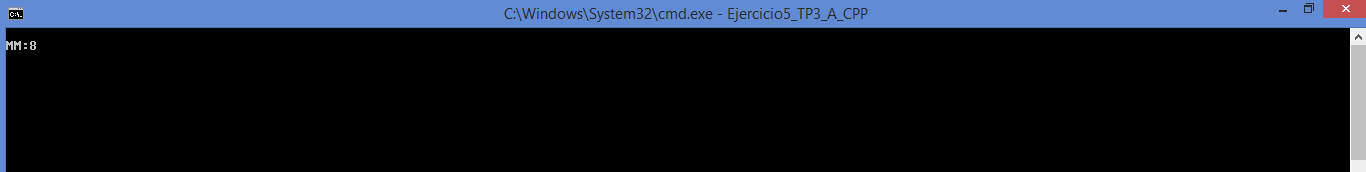
\includegraphics{Captura_UI_5.PNG}
    \end{adjustbox}
    \begin{adjustbox}{max width=\textwidth, center}
        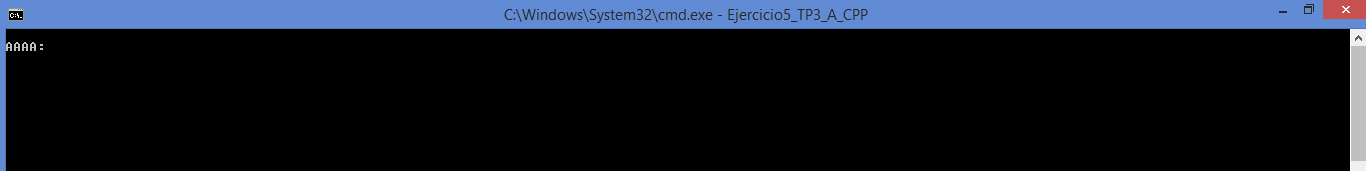
\includegraphics{Captura_UI_6.PNG}
    \end{adjustbox}
    \begin{adjustbox}{max width=\textwidth, center}
        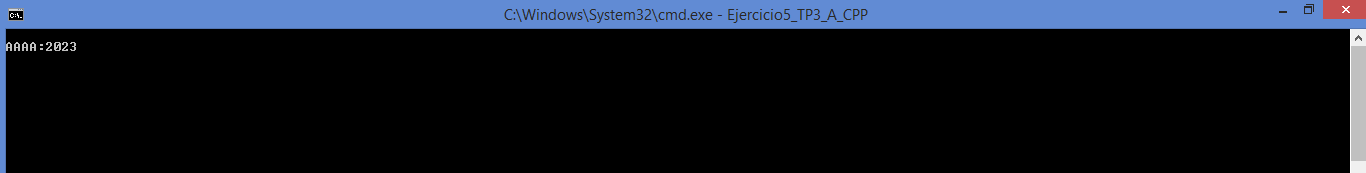
\includegraphics{Captura_UI_7.PNG}
    \end{adjustbox}
    \begin{adjustbox}{max width=\textwidth, center}
        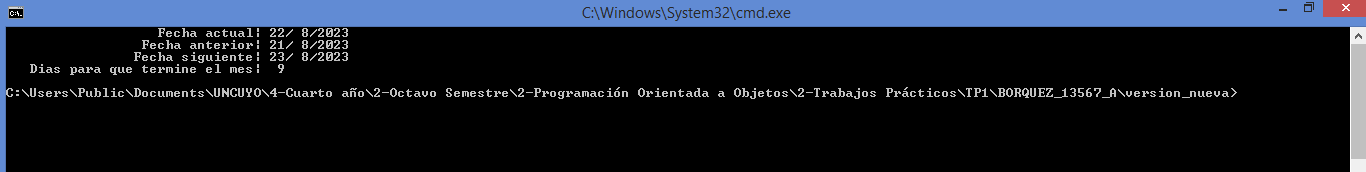
\includegraphics{Captura_UI_8.PNG}
    \end{adjustbox}
\end{figure}
\newpage
\section{Uso}

La aplicación que se presenta permite la obtención de la fecha anterior, de la fecha siguiente y de la cantidad de días para la conclusión del mes de cualquier fecha del calendario gregoriano indicada por el usuario.

Se consideran como fechas válidas únicamente aquellas que corresponden al calendario gregoriano y por lo tanto son posteriores al 15 de Octubre de 1582 (15/08/1582). Sin embargo, por cuestiones de simplicidad del código, solamente se consideran como válidas una fecha igual o posterior al 1 de Noviembre de 1582 (01/09/1582).

En la ejecución del código se pide al usuario que ingrese el día, el mes y el año de la fecha. En cada entrada de dato se realiza una verificación cíclica. Si se ingresa un número de día erróneo (por ejemplo, un número menor a 1 o mayor a 31, o un valor no numérico), la aplicación solicitará repetidamente un nuevo valor para el día hasta que se ingrese un valor correcto. El mismo proceso se aplica para el mes y el año. Si después de verificar cada dato individual, la fecha en conjunto es errónea debido a que no pertenece al calendario gregoriano, la aplicación también solicitará repetidamente el ingreso de nuevos datos de fecha hasta que se ingrese una fecha válida en su conjunto.

Tenga en cuenta que la aplicación presenta un error: si en el prompt para un dato de la fecha se presiona la tecla "ENTER" antes de introducir un dato numérico (o un carácter alfabético), la aplicación se bloqueará.
\section{Conclusiones}
\subsection{Cambios Realizados en el Código de la Aplicación}

La mayoría de los cambios realizados en el código se encuentran indicados en el código fuente de la aplicación como comentarios de línea. Otros de los cambios realizados son los siguientes:

\begin{itemize}
    \item Los datos de la fecha no se asignan directamente a la estructura de la fecha (la que tiene todos los campos numéricos) y en cambio se lleva a cabo una verificación previa de que los datos ingresados por el usuario sean numéricos. Para ello, se realiza el siguiente cambio.
    \item Incorporación de funciones para la verificación de los datos de una fecha dados en un string:
    \begin{itemize}
        \item \texttt{bool valid\_DD(char* DD);}
        \item \texttt{bool valid\_MM(char* MM);}
        \item \texttt{bool valid\_AAAA(char* AAAA);}
    \end{itemize}
    \item Incorporación de una función que concentra la muestra de los resultados de la ejecución:
    
     \texttt{void print\_out(Date current,Date previous,Date next,short int days\_MM);}
    \item Se realizaron cambios en la presentación de algunas funciones y correcciones por fallas encontradas en la lógica del programa.
\end{itemize}

\subsection{Dificultades Encontradas}

Se utilizó la siguiente forma de tomar los datos de la fecha:

\begin{verbatim}
cin.get(auxiliar, 3);
\end{verbatim}

De esta manera, se almacena en la variable "auxiliar" como máximo dos caracteres de los ingresados por el usuario (para el caso del mes y del día, mientras que son 4 para el caso del año). Si el usuario ingresa más de 2 caracteres antes de presionar "ENTER", el resto de los caracteres en el buffer de entrada son consumidos por la siguiente línea:
\begin{verbatim}
cin.ignore(numeric_limits<streamsize>::max(), '\n');
\end{verbatim}
El problema se presenta cuando el usuario no ingresa ningún carácter antes de presionar "ENTER". En este caso, el programa se bloquea en el ciclo \texttt{do{} while}, ya que aparentemente queda en el buffer de entrada un carácter no imprimible. Esto se pudo determinar por pruebas imprimiendo por pantalla el código ASCII del carácter obtenido del buffer de entrada.

\section{Referencias Bibliográficas}
\cite{cplusplus-setw}, \cite{geeksforgeeks-setw}, \cite{geeksforgeeks-input-buffer}, \cite{cplusplus-stoi}, \cite{geeksforgeeks-stoi}, \cite{stackoverflow-cin-get}, \cite{geeksforgeeks-cin-get}

\printbibliography[title={Referencias}]

\end{document}